\begin{lstlisting}
    cronometro SO;
    long int r1 = 0;
    const double e_abs = 0.01, e_rel = 0.001;
    SO.activar();
    do {
        placeDefenses_SO(freeCells, nCellsWidth, nCellsHeight, mapWidth, mapHeight, obstacles, defenses);
	++r1;
    } while(SO.tiempo() < e_abs / e_rel + e_abs);
    SO.parar();

    cronometro OR;
    long int r2 = 0;
    OR.activar();
    do {
        placeDefenses_OR(freeCells, nCellsWidth, nCellsHeight, mapWidth, mapHeight, obstacles, defenses);
	++r2;
    } while(OR.tiempo() < e_abs / e_rel + e_abs);
    OR.parar();

    cronometro F;
    long int r3 = 0;
    F.activar();
    do {
        placeDefenses_F(freeCells, nCellsWidth, nCellsHeight, mapWidth, mapHeight, obstacles, defenses);
	    ++r3;
    } while(F.tiempo() < e_abs / e_rel + e_abs);
    F.parar();
    
    cronometro M;
    long int r4 = 0;
    M.activar();
    do {
        placeDefenses_M(freeCells, nCellsWidth, nCellsHeight, mapWidth, mapHeight, obstacles, defenses);
	    ++r4;
    } while(M.tiempo() < e_abs / e_rel + e_abs);
    M.parar();
    std::cout << (nCellsWidth * nCellsHeight) << "\t" << SO.tiempo() / r1 << "\t" << F.tiempo() / r3 << "\t" << OR.tiempo() / r2 << "\t" << M.tiempo() / r4 << std::endl;
\end{lstlisting}
\begin{center}
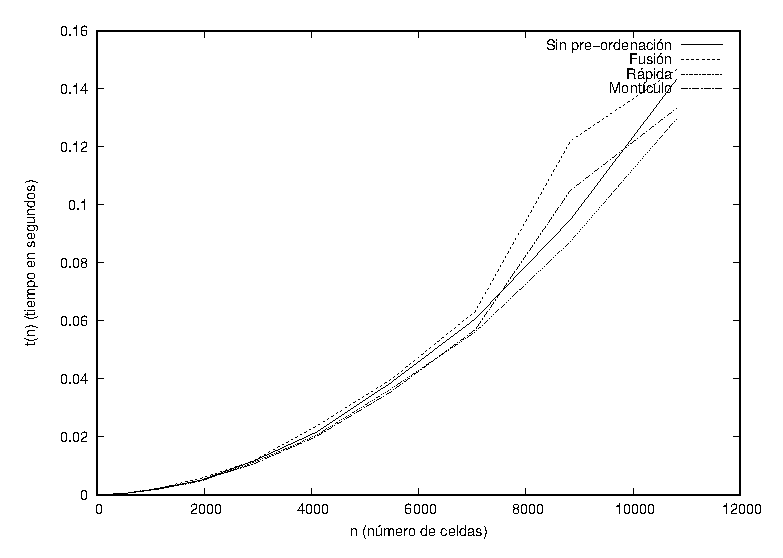
\includegraphics[scale=0.9]{graphic.eps} 
\end{center}